\documentclass[12pt, a4paper]{article}

% Formatting Requirements
\usepackage[margin=1in]{geometry}
\usepackage{fontspec}
\usepackage{titlesec}
\usepackage{setspace}
\usepackage{graphicx}
\usepackage{hyperref}
\usepackage[document]{ragged2e} % For justified alignment

% Font and Spacing Setup
\setmainfont{Times New Roman}
\setstretch{1.5}
\hyphenpenalty=10000

% Heading Formatting
\titleformat{\section}{\fontsize{16}{18}\bfseries}{\thesection}{1em}{}
\titleformat{\subsection}{\fontsize{14}{16}\bfseries}{\thesubsection}{1em}{}

\begin{document}

% Cover Page
\begin{titlepage}
    \begin{center}
        \vspace*{2cm}
        
        {\fontsize{24}{28}\bfseries Analyzing the Role of AI-Assisted Programming in Modern Software Development}\\[0.8cm]
        
        {\fontsize{14}{16} \textbf{IT3003} : Advanced Programming Techniques}\\[2cm]
        
        \textbf{Submitted By :}\\[0.2cm]
        {\fontsize{14}{16} Name : D.Harishun}\\
        {\fontsize{14}{16} Student ID : s17223}\\
        {\fontsize{14}{16} Registration No : 2023s19951}\\[3cm]

        \textbf{Faculty of Science}\\
        \textbf{University of Colombo}\\[0.2cm]
        
        \vfill
        
        \textbf{Date:}\\[0.2cm]
        {\fontsize{14}{16} \today}\\[1cm]
    \end{center}
\end{titlepage}
\newpage

\section{Introduction}
Artificial Intelligence is increasingly integrated into modern software development through tools
such as AI code generators, debugging assistants, and intelligent programming support systems.
These technologies are transforming how developers design, implement, test, and maintain
software applications. This study aims to test the pros and cons and the extremes of traditional and AI assisted programming.

\section{Conceptual Understanding}
\subsection{AI-Assisted Programming}
AI-Assisted Programming is the integration of artificial intelligence tools into the software development lifecycle to support developers in planning, designing, implementing, testing, and maintaining applications.
This allows the programmer to oversee the development process and audit the code without manually writing every single line of code by hand. This tools work by predicting the next words and eventually writing a program. This is done by a statistical model trained on already available code. Which then allows the AI-Tool to predict what word is highly likely to appear next.
This is similar to the quote "Give 1000 monkeys a type writter and a very long time and they'll eventualy write the entire work of Shakesphere". Even though it says that the randomn keystrokes produce a pattern over time, the statistical model is also similar. Think of it as the monkeys learn the pattern and overtime they learn what word is mostlikely to appear next. This is how code completion and code generation work behind the scene.

\subsection{Types of AI Coding Tools}
Since we are in the age of AI, there are lot of paid, free, closesource and opensource tools out there. But the main types of tools used in programming are as follows.
\begin{itemize}
    \item \textbf{Code Completion} : These types of tools allows the user to start typing the structure of the code and the tool will suggest the best solution that it thinks suits the best.
    \item \textbf{Code Generation} : These types of tools allows the user to describe the feature or the programm and the tool will generate the entire code base.
    \item \textbf{Code Debugging} : These tools run automated tests and generate test cases to test possible scenarios to ensure the program produces reliable and consistent results. And this helps you find bugs in the code.
    \item \textbf{Code refactoring} : These tools help the user to rewrite the program after reaching a functional stage to make the code readable.
    \item \textbf{AI Agents} : These tools are the most feature packed ones. These allow the user to describe what they want and the Agents do research, plan, design, build, test, debug and maintain the code base. Even though this is better than the individual tools, it still needs a human in the loop. This ensures that the AI is on the right path, and sticks to what you intended. This is done by getting approval from the user at every stage.
\end{itemize}

\subsection{Advantages in Software Development}
\begin{itemize}
    \item \textbf{Easy Entry into Software Engineering} : With the use of AI tools, even those who don't know programming can create software solution to a problem at a low cost.
    \item \textbf{Low Resource Production} : Since most of the tedious tasks are done by the AI tools, This allows a single or limited amount of developers to produce an enterprise grade software, which usually takes a big team.
    \item \textbf{Fast Development} : The existance of AI tools allow the user to prototype rapidly and make production grade software, quicker than it used to.
\end{itemize}

\subsection{Risks and Limitations}
\begin{itemize}
    \item \textbf{Hallucination} : Since the model is trained on every available resource, which might include faulty code and codes which don't follow coding best practices. When genreating code even though the next probable word might be something, that doesn't necessarily mean the code is syntactically correct or functionally correct. Which leads to hallucinated unrelated predictions.
    \item \textbf{Security} : When you use an AI tool, it most likely sends your code to be trained on. This exposes the unencrypted plain text passwords or API keys or even encryption keys to the public. Since it was trained on your code as well, when another person is trying to generate code it might provide your API key to that code. And also if you don't read and understand the code before implementing the program, the program might run malicious code generated by the tool.
\end{itemize}

\newpage
\section{System Design and UML Diagrams}
To evaluate the refactoring process and comparative programming, we developed a Library Management System using two approaches: a manually refactored design based on strict object-oriented delegation patterns, and an entirely AI-generated system. The architectures of these systems are modeled through the following UML diagrams.

\subsection{Use Case Diagram}
The Use Case Diagram (Figure \ref{fig:usecase}) models the system actors (User, Administrator, and Library System) and their associated interactions. It depicts how members register, search, borrow, return books, and pay fines, alongside the librarian administrative features.

\begin{figure}[htbp]
    \centering
    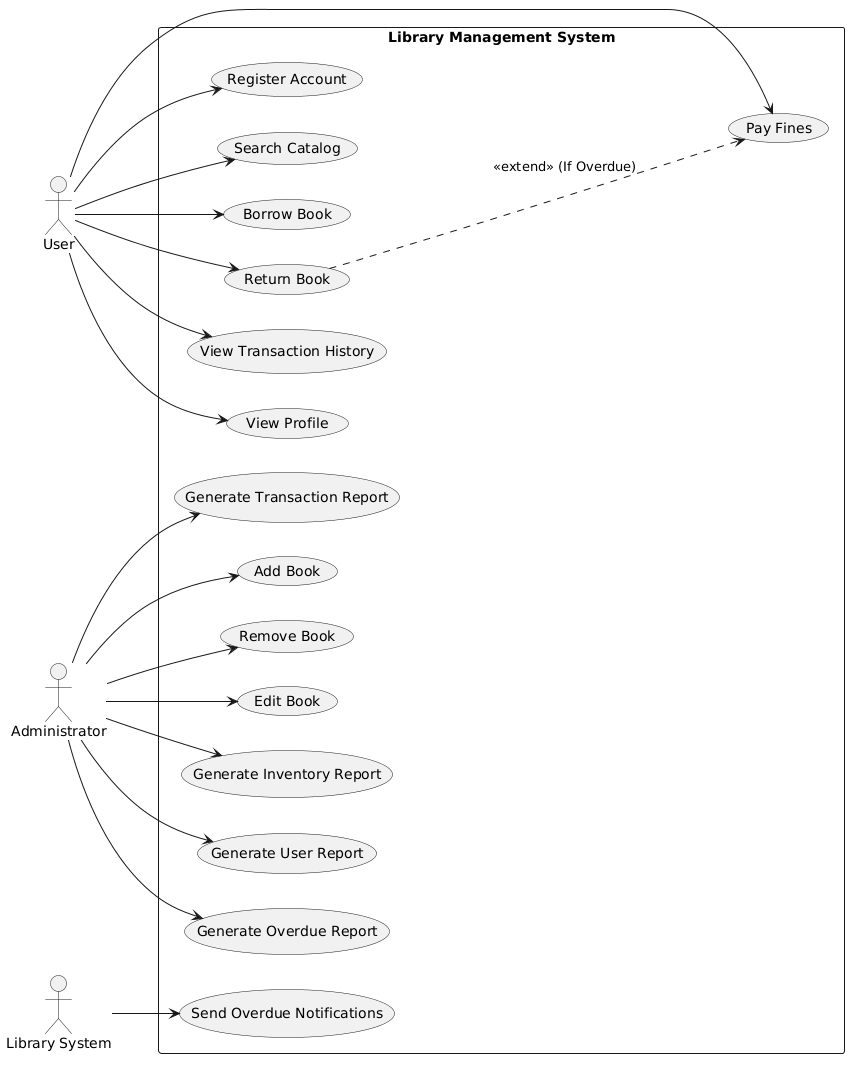
\includegraphics[width=0.75\textwidth]{useCase.png}
    \caption{Library System Use Case Diagram}
    \label{fig:usecase}
\end{figure}

\subsection{Class Diagram}
The Class Diagram (Figure \ref{fig:classdiagram}) details the structural dependencies, properties, and method signatures of the system entities (User, Member, Administrator, Book, and Transaction) and the main DigitalLibrary coordinator class. It emphasizes the static `searchBook` method design.

\begin{figure}[htbp]
    \centering
    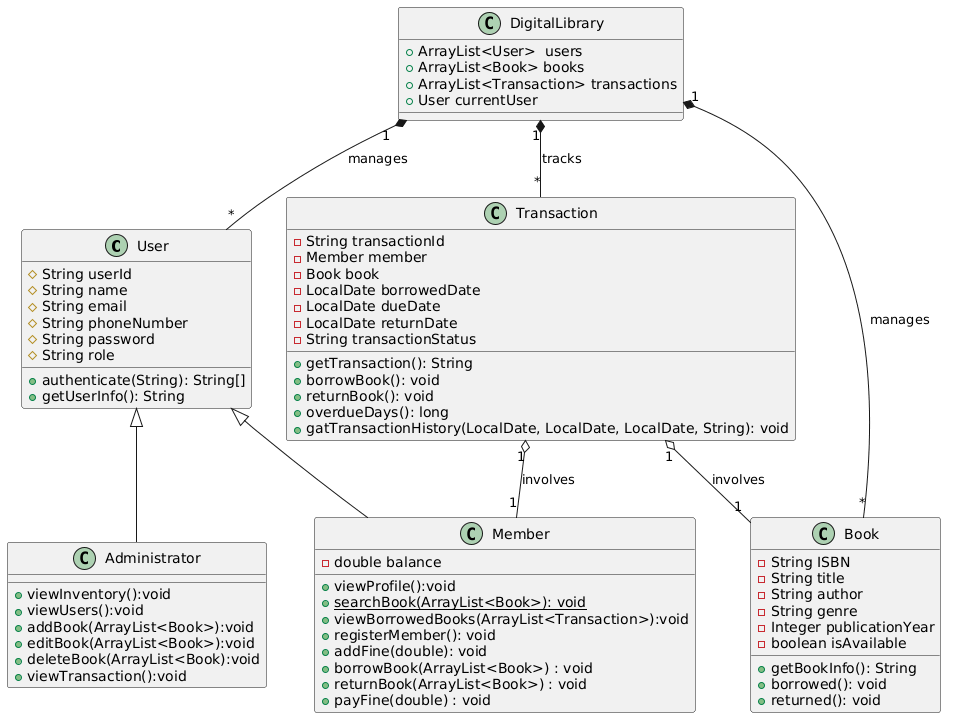
\includegraphics[width=0.85\textwidth]{classDiagram.png}
    \caption{Library System Class Diagram}
    \label{fig:classdiagram}
\end{figure}

\newpage
\subsection{Activity Diagram}
The Activity Diagram (Figure \ref{fig:activitydiagram}) details the dynamic flow of control from the initial user login to the dashboard menus, showing the branching logic for borrowing checks, fine payments, returns, and librarian actions.

\begin{figure}[htbp]
    \centering
    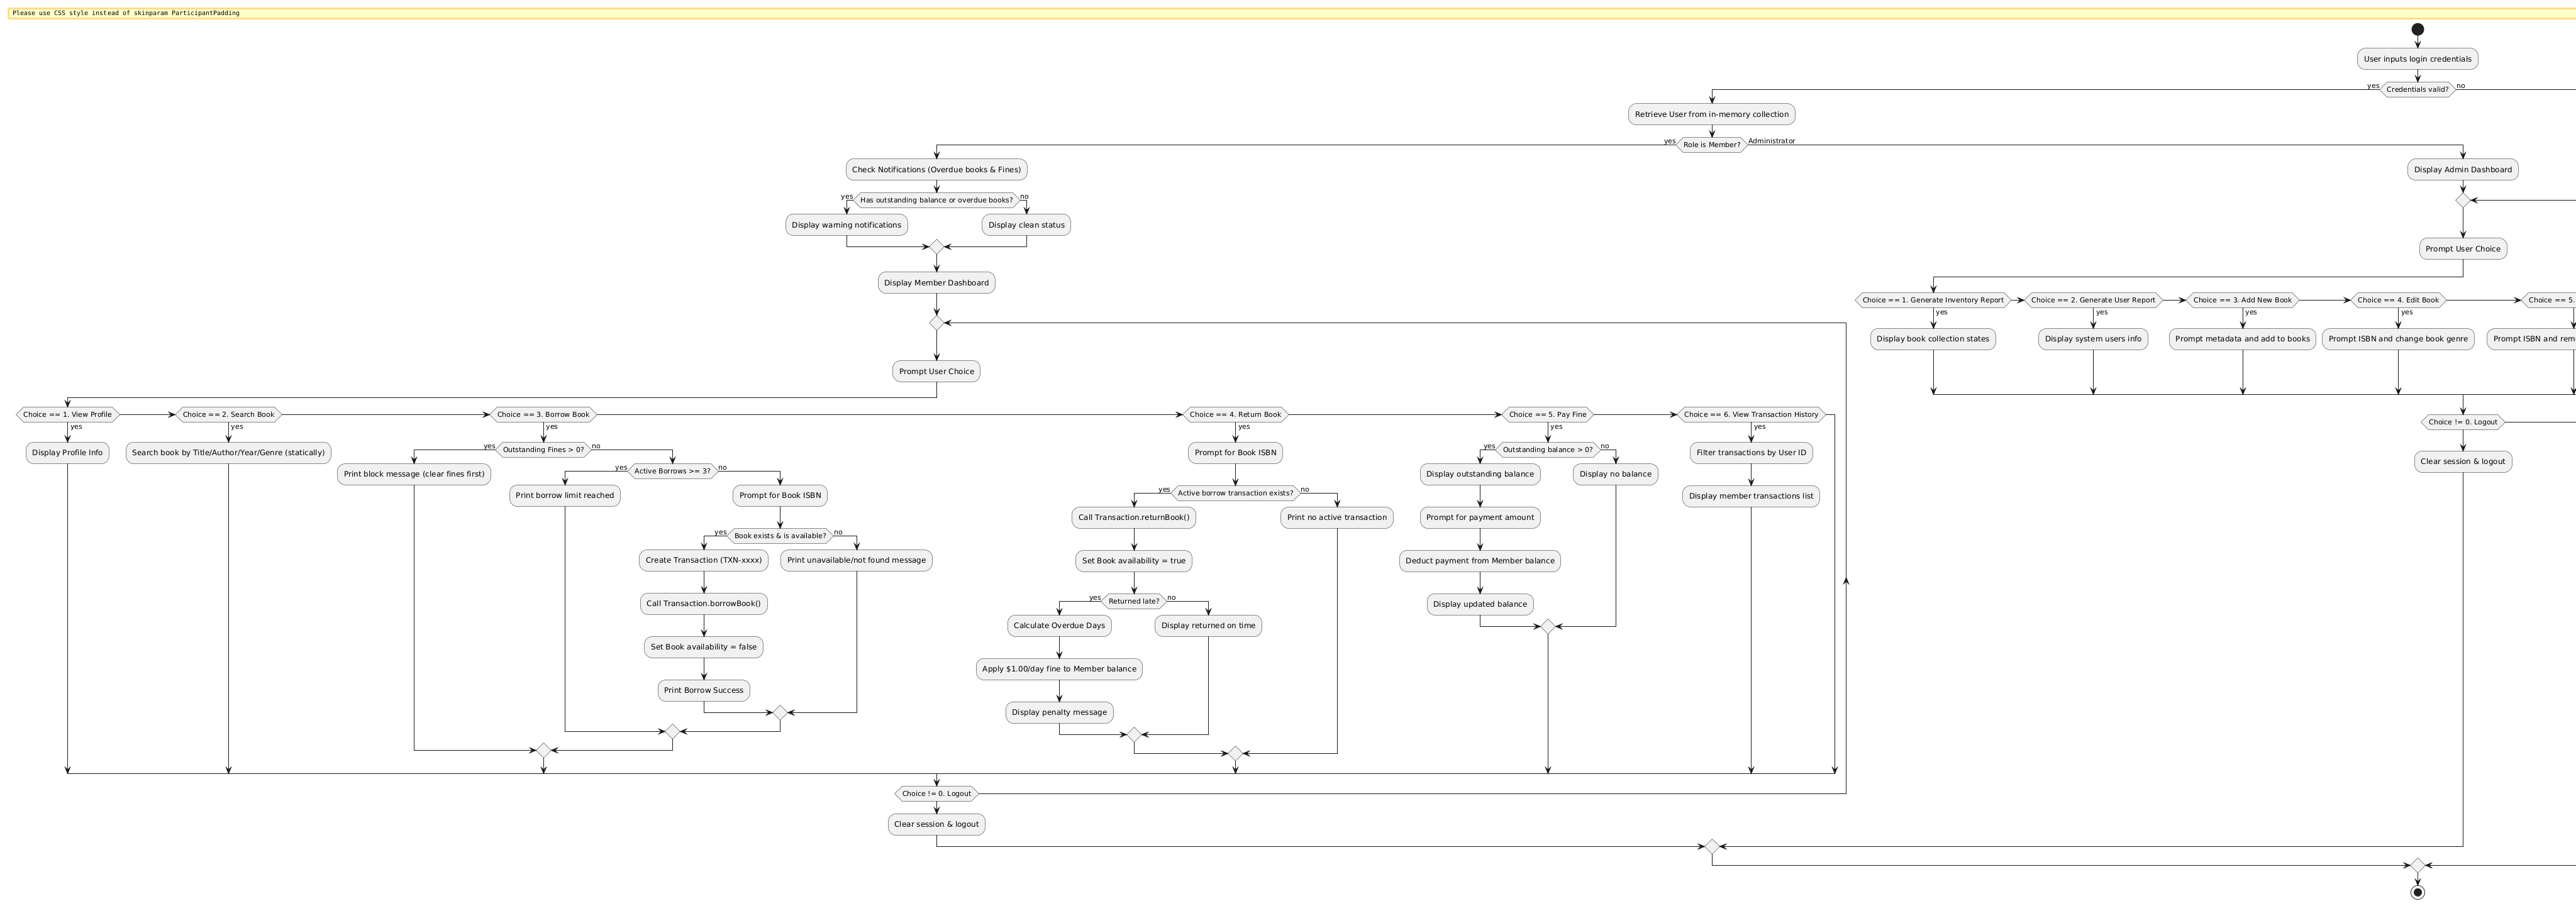
\includegraphics[width=0.75\textwidth]{activityDiagram.png}
    \caption{Library System Activity Workflow Diagram}
    \label{fig:activitydiagram}
\end{figure}

\subsection{Sequence Diagram}
The Sequence Diagram (Figure \ref{fig:sequencediagram}) details the message passing involved when a member borrows a book, highlighting the delegation of validation and borrow state updates to the Member instance.

\begin{figure}[htbp]
    \centering
    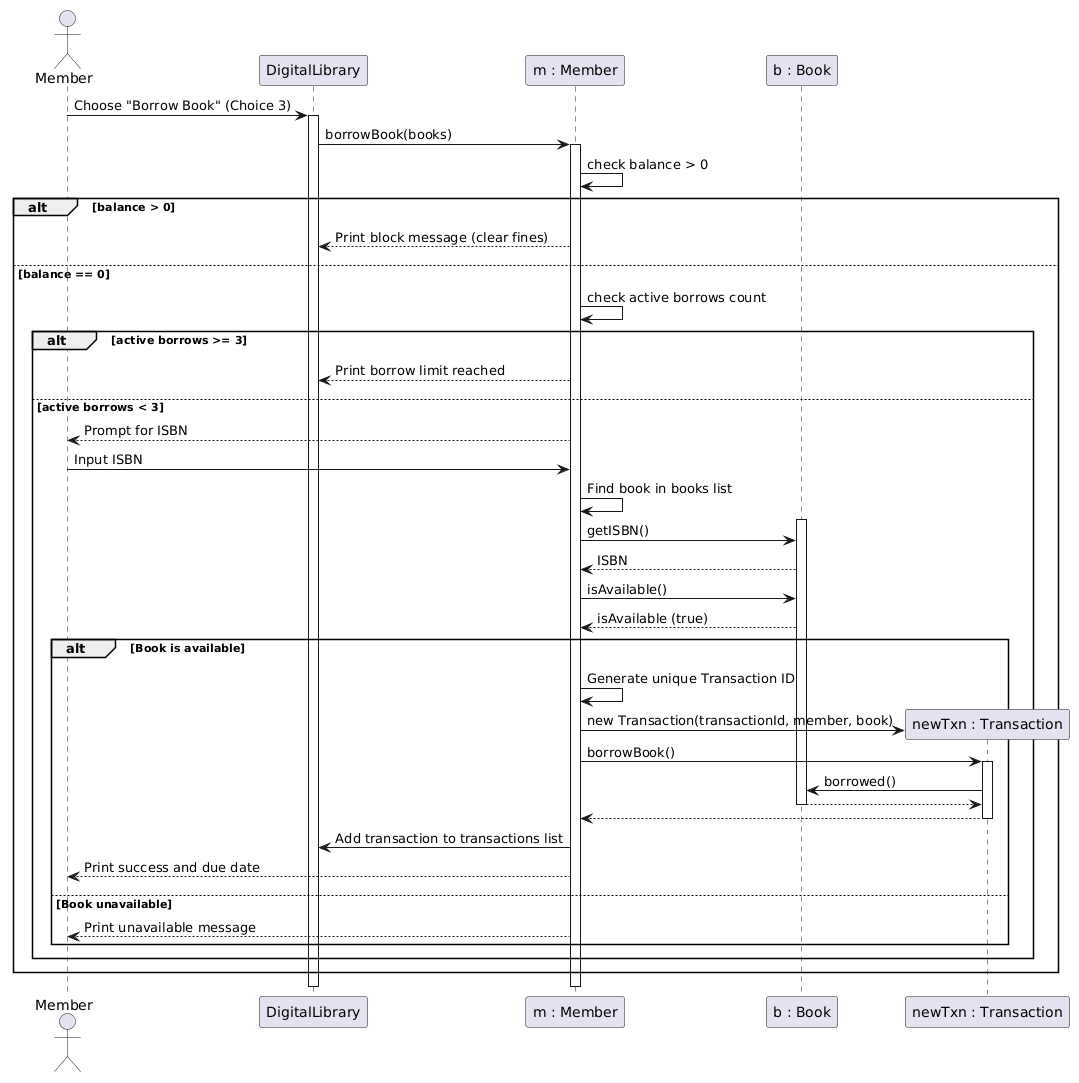
\includegraphics[width=0.8\textwidth]{sequenceDiagram.png}
    \caption{Book Borrowing Sequence Diagram}
    \label{fig:sequencediagram}
\end{figure}

\newpage
\section{Project Implementation and Source Code}
The project source code is organized into two complete versions located within the project repository:
\begin{enumerate}
    \item \textbf{Manual Library System}: Located in the \texttt{Manual\_Library\_System} directory. This version strictly implements the class diagram structure with manual refactoring, utilizing class delegation and getRole checks.
    \item \textbf{AI Library System}: Located in the \texttt{AI\_Library\_System} directory. This is an entirely AI-generated system with package packaging, in-memory processing with flat-file database persistence, and system-wide overdue notifications.
\end{enumerate}

All code, UML files, and compiled artifacts are managed in the Git repository.

\subsection{GitHub Repository Link}
The complete codebase, reports, and UML diagrams are hosted and open-sourced on GitHub. You can view and clone the project at the following address:
\begin{center}
    \url{https://github.com/harishun/Digital_Library}
\end{center}

\end{document}